\documentclass[a4paper, french]{article}
\usepackage{config}
\author{Vincent Commin \& Louis Leenart}
\date{\today}
\setcounter{secnumdepth}{6}
\begin{document}

\begin{titlepage}
    \begin{flushleft}
        \includegraphics[width=5cm]{UL.jpg}\par
        \centering

        \vspace{13\baselineskip}
        \HRule \\[0.4cm]

        {\Huge
        GIF-4104 - TP 4\par}
        \vspace{0.4cm}
        \HRule
        \vfill
        Équipe 1 : Vincent Commin \& Louis Leenart\medskip \par
    \end{flushleft}
\end{titlepage}

\newpage
\section{Introduction}

Pour ce quatrième TP, nous avons implémenté la parallélisation d'inversion d'une matrice en utilisant
méthode de \href{https://fr.wikipedia.org/wiki/%C3%89limination_de_Gauss-Jordan}{\textit{\underline{Gauss Jordan}}}
avec  \href{https://www.khronos.org/opencl/}{\textit{\underline{OpenCL}}} et \href{https://www.openacc.org/}{\textit{\underline{OpenACC}}}. En se basant sur l'implémentation séquentielle proposée, nous avons suivi l'approche par réduction puis diffusion successives.

\section{Notre approche}

\subsection{OpenCL}

Dans ce TP, nous avons découvert l'utilisation d'OpenCL ainsi que ses particularités. En implémentant l'algorithme d'inversion de matrix de Gauss Jordan pour une architecture de GPU, nous avions en tête de diminuer le temps de calcul pour qu'il soit inférieur à celui obtenu avec l'utilisation uniquement du CPU.

L'algorithme que nous avons mis en place est le suivant :

\begin{lstlisting}[style=txt]
AI : Matrix [A I] // Shared amoung every GPU threads
Buffer : value array // Shared amoung every GPU
size, rank : integer

FOR k = 0 TO AI.rows DO
    max = 0, pivotIndex = k
    FOR i = k TO AI.rows DO // Find greatest pivot for column k
        IF (i mod size) == rank && abs(AI[i, k]) > max DO
            max = abs(AI[i, k]); pivotIndex = i
        DONE
    DONE

    Buffer[pivotIndex] = max
    pivotIndex = Reduce(MAX_LOG, Buffer) // Location of max value in Buffer

    IF IA[pivotIndex, k] == 0 DO throw exception DONE

    v = AI[k, k] // Normalisation
    FOR j = 0 TO AI.cols DO
        AI[k, j] = AI[k, j] / v
    DONE

    FOR i = 0 TO AI.rows DO // For each rows
        IF i mod size == rank && i != k DO
            AI[i] -= AI[k] * AI[i, k]
        DONE
    DONE
DONE

FOR i = 0 TO AI.rows DO // Copy right side of AI into result
    A = AI.getData()[slice(i * AI.cols + AI.rows, AI.rows, 1)]
DONE
\end{lstlisting}

\subsection{OpenACC}

% TODO(Vincent)

\section{Machine utilisée pour les tests de performance}

\begin{center}
    \begin{tabularx}{0.6\textwidth}{|>{\raggedleft\arraybackslash}X|>{\raggedright\arraybackslash}X|}
        \hline
        Modèle & intel i7-8550U \\
        \hline
        Architecture & x86\_64 \\
        \hline
        OS & Archlinux \\
        \hline
        Fréquence CPU & 3.4GHz \\
        \hline
        C\oe urs physiques & 4 \\
        \hline
        Ram & 16 Go, 2400 $MT/s$ \\
        \hline
        GPU & Intel(R) UHD Graphics 620 \\
        \hline
        OpenCL & version \textbf{3.0} \\
        \hline
        GCC & version \textbf{11.2.0} \\
        \hline
        nvc++ & version \textbf{22.1} \\
        \hline
    \end{tabularx}
\end{center}

\section{Résultats obtenus}

\begin{center}
    \begin{tabularx}{\textwidth}{c c}
        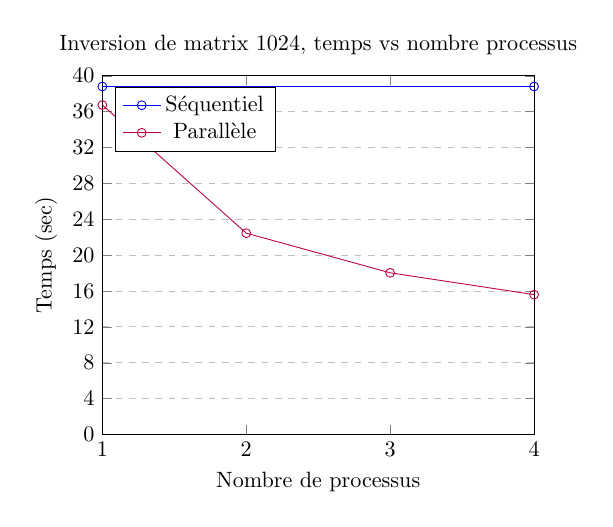
\begin{tikzpicture}[scale=0.8, transform shape]
            \begin{axis}[
                title={Inversion de matrix 1024, temps vs nombre processus},
                xlabel={Nombre de processus},
                ylabel={Temps (sec)},
                xmin=1, xmax=4,
                ymin=0, ymax=40,
                xtick={1, 2, 3, 4},
                ytick={0, 4, 8, 12, 16, 20, 24, 28, 32, 36, 40},
                legend pos=north west,
                ymajorgrids=true,
                grid style=dashed,
                ]
                \addplot[color=blue, mark=o] coordinates {(1, 38.8119)(4, 38.8119)};
                \addplot[color=purple, mark=o] coordinates {(1, 36.7437)(2, 22.4539)(3, 18.0343)(4, 15.5994)};

                \legend{Séquentiel, Parallèle}
            \end{axis}
        \end{tikzpicture}
        &
        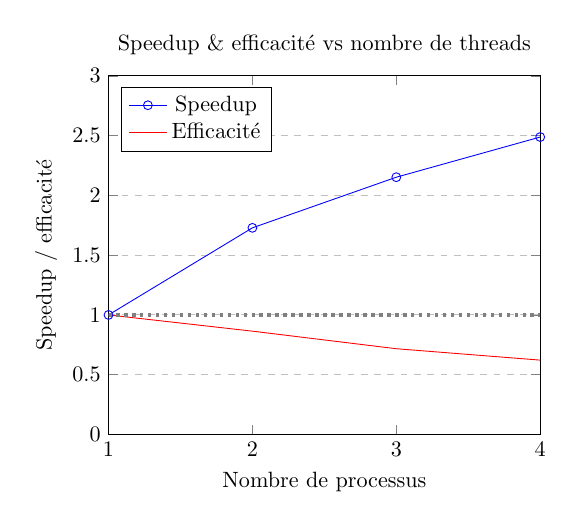
\begin{tikzpicture}[scale=0.8, transform shape]
            \begin{axis}[
                title={Speedup \& efficacité vs nombre de threads},
                xlabel={Nombre de processus},
                ylabel={Speedup / efficacité},
                xmin=1, xmax=4,
                ymin=0, ymax=3,
                xtick={1,2,3,4},
                ytick={0, 0.5, 1, 1.5, 2, 2.5, 3},
                legend pos=north west,
                ymajorgrids=true,
                grid style=dashed,
                ]
                \addplot[color=blue, mark=o] coordinates {(1, 1)(2, 1.728514868)(3, 2.152115691)(4, 2.488038001)};
                \addplot[color=red, mark=] coordinates {(1, 1)(2, 0.8642574341)(3, 0.7173718969)(4, 0.6220095004)};
                \addplot[color=gray, dotted, ultra thick] coordinates {(0, 1)(8, 1)};
                \legend{Speedup, Efficacité}
            \end{axis}
        \end{tikzpicture}
    \end{tabularx}
\end{center}

\newpage

\section{Analyse}

Tout d'abord, nous avons conduit notre analyse sur l'inversion de matrices de tailles variées. Les
résultats ayant la même tendance par rapport à la taille, nous avons décidé de nous concentrer seulement
sur l'inversion d'une matrice 1024x1024 aléatoire (les données brutes pour d'autres tailles sont
disponibles) dans l'archive.

L'utilisation de MPI, en contraste avec OpenMP, permet d'établir un environnement de travail spécifique
à chaque processus de calcul. En effet, pour que deux processus communiquement, il ne faut plus simplement
appeler une fonction, il faut faire une transmission de message. Une des méthodes de transmission de message
s'appelle le `Broadcast' et est particulièrement couteuse étant donné quelle fait appel à tous les processus.
MPI possède de nombreux moyens de transmettre et reçevoir des messages, cependant, le `Broadcast' est ce que
nous avons utilisé pour notre algorithme.

Pour en revenir aux performances de notre algorithme, nous pouvons remarquer avec le premier graphique
que le temps de calcul pour une matrice 1024 décroit comme attendu quand le nombre de processus augmente.
Ce comportement est celui attendu étant donné le travail de parallélisation. De plus, on note que le temps
de calcul initial est assez conséquent (environ 40 secondes), et le minimum obtenu pour 4 processus est
autour de 16 secondes. Ces résultats sont satifsaisants, mais nous pouvons étudier le speedup et l'efficacité
pour mieux comprendre les gains en performance.

D'après le graphique, on remarque que pour 4 processus, le speedup atteint 2.5 ce qui est non négligeable pour
une application parallèle. De plus, l'efficacité atteint 0.6 pour 4 processus, ce qui n'est pas particulièrement
impressionnant, mais cela reste correct. On peut donc en déduire que la parallélisation de l'algorithme d'inversion
de matrice selon la méthode de Gauss Jordan est fonctionnelle.

Cependant, il est évident que l'approche naïve du problème ne nous permet pas d'utiliser le plein potentiel de
parallélisation. En effet, il existe au moins une autre approche pour cette algorithme, dite par "répartition
cyclique" ou par "pipeline" permettant d'éliminer un maximum les temps d'attente des processus imposés par notre
approche.

\section{Conclusion}

Avec la prise en main de MPI, nous avons pu mettre en pratique une nouvelle approche de la parallélisation de
calculs. Dans un premier temps, nous nous sommes lancés sur l'implémentation de la méthode naïve pour l'algorithme
de Gauss Jordan, avec succès. Même si les résultats se sont montrés satifsaisants, nous avons tenté de mettre en
place l'algorithme par pipeline, mais rattrapés par le temps, nous n'avons pas eu le temps de l'achever.

Cependant, la méthode de Gauss Jordan n'est pas la seule façon d'inverser une matrice. Par exemple, la méthode de
\href{https://en.wikipedia.org/wiki/Cayley%E2%80%93Hamilton_theorem}{\textit{\underline{Cayley-Hamilton}}} dont la formule se résume à :\newline
$A^{-1}=\frac{1}{det(A)}\sum_{k_1, k_2,...,k_n}^{}\prod_{n-1}^{l=1}\frac{(-1)^{k_l+1}}{l^{k_l}k_l!}tr(A^l)^{k_l}$
\newline
Aussi, pour les matrices dites \href{https://en.wikipedia.org/wiki/Definite_matrix}{\textit{\underline{positive definite}}},
l'application de la décomposition de \href{https://en.wikipedia.org/wiki/Cholesky_decomposition}{\textit{\underline{Cholesky}}},
avec la formule suivante:
$A^{-1}=(L^*)^{-1}L^{-1}$
\end{document}